\subsection{Niveau 2 - Tazer}

\begin{center}
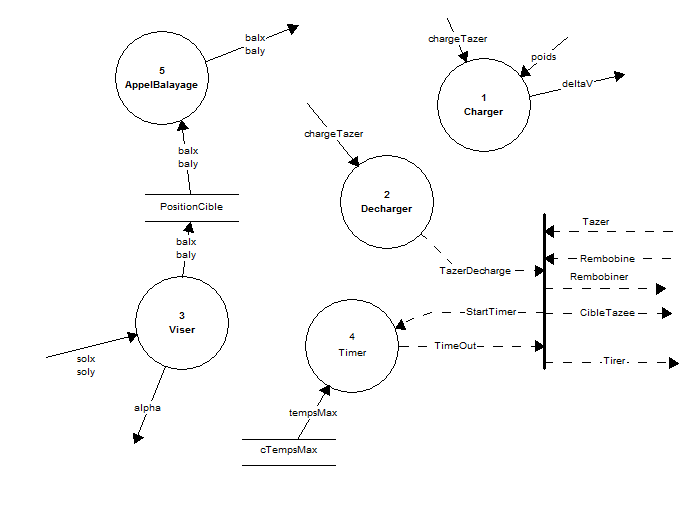
\includegraphics[scale=0.8]{\PIXPATH/tazer}
\end{center}


\subsubsection{Diagramme état-transition}

\begin{center}
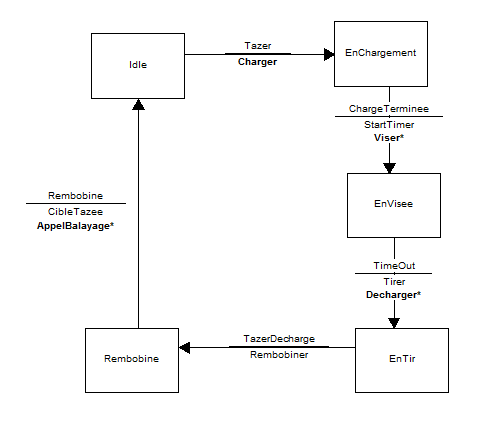
\includegraphics[scale=0.8]{\PIXPATH/tazer_etat}
\end{center}

\vfill
\pagebreak

\subsubsection{Processus primitifs - C-Spec}

\begin{description}
	
	\item \textbf{Charger}
		\begin{tabbing} 
		\textbf{IN} : chargeTazer, poids \\
		\textbf{OUT} : deltaV, ChargeTerminee \\
		deltaV : poids * 200 \\	
		si \=($chargeTazer \geq deltaV$) alors \\
			\>ChargeTerminee emis \\
		fin si
		\end{tabbing}

	\item \textbf{Decharger}
		\begin{tabbing} 
		\textbf{IN} : chargeTazer \\
		\textbf{OUT} : TazerDecharge \\
		si \=($chargeTazer \leq 0$) \\
			\>TazerDecharge emis \\
		fin si
		\end{tabbing} 

	\item \textbf{Viser}
		\begin{tabbing} 
		\textbf{IN} : solx, soly \\
		\textbf{OUT} : balx, baly, alpha \\
		alpha : $\arctan(\frac{soly}{solx})$ \\
		balx : solx \\
		baly : soly
		\end{tabbing} 

	\item \textbf{AppelBalayage}
		\begin{tabbing} 
		\textbf{IN} : balx, baly \\
		\textbf{OUT} : balx, baly \\
		balx : balx \\
		baly : baly
		\end{tabbing} 

\end{description}

\vfill
\pagebreak


